% !TeX root = main.tex

\hypertarget{optimization-problems}{%
\section{Optimization Problems}\label{optimization-problems}}

\hypertarget{optimization-problem-solving-strategy}{%
\subsection{Optimization Problem Solving
Strategy}\label{optimization-problem-solving-strategy}}

\begin{enumerate}
\item
  Understand the Problem and represent known and unknown quantities
  using variables and expressions. In this step, it is useful to draw a
  diagram and identify variables and expressions on the diagram.
\item
  Write equations relating the variables.
\item
  Determine which quantity is to be maximized or minimized. Find the
  range of values of the other variables if possible.
\item
  Express the quantity to be maximized or minimized as an explicitly
  define function of other variables.
\item
  Locate the maximum or minimum value of the function.
\end{enumerate}

\begin{example}

A rectangular garden is to be constructed using a rock wall as one side
of the garden and wire fencing for the other three sides. Given \(100\)
ft of wire fencing, determine the dimensions that would create a garden
of maximum area. What is the maximum area?

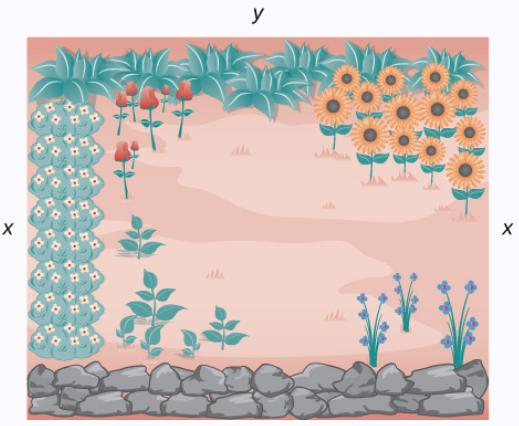
\includegraphics[width=0.9\textwidth]{img/image-20200420233408884.png}

\end{example}
\vspace*{6\baselineskip}

\begin{example}

An open-top box is to be made from a \(24\) in. by \(36\) in. piece of
cardboard by removing a square from each corner of the box and folding
up the flaps on each side. What size square should be cut out of each
corner to get a box with the maximum volume?

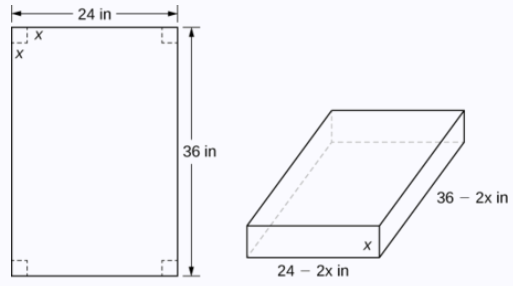
\includegraphics[width=0.9\textwidth]{img/image-20200420233831196.png}

\end{example}
\vspace*{6\baselineskip}

\begin{example}

An island is \(2\,mi\) due north of its closest point along a straight
shoreline. A visitor is staying at a cabin on the shore that is
\(6\,mi\) west of that point. The visitor is planning to go from the
cabin to the island. Suppose the visitor runs at a rate of \(8\,mph\)
and swims at a rate of \(3\,mph\). How far should the visitor run before
swimming to minimize the time it takes to reach the island?

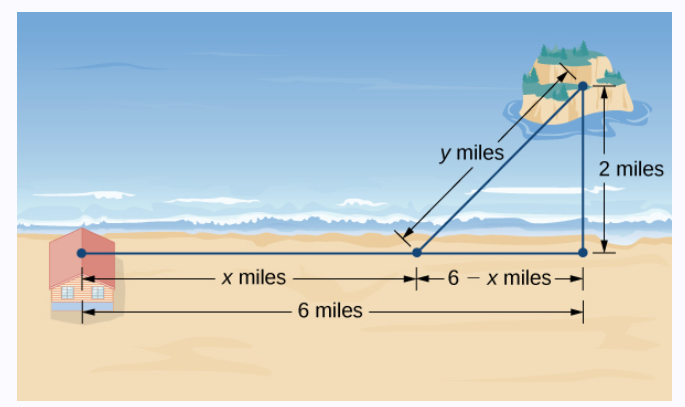
\includegraphics[width=0.9\textwidth]{img/image-20200420234008040.png}

\end{example}
\vspace*{6\baselineskip}

\begin{example}

Owners of a car rental company have determined that if they charge
customers \(p\) dollars per day to rent a car, where \(50 \le p \le 200\), the
number of cars \(n\) they rent per day can be modeled by the linear
function \(n(p)=1000 - 5p\). If they charge \(\$50\) per day or less, they
will rent all their cars. If they charge \(\$200\) per day or more, they
will not rent any cars. Assuming the owners plan to charge customers
between \(\$50\) per day and \(200\) per day to rent a car, how much
should they charge to maximize their revenue?

\end{example}
\vspace*{6\baselineskip}

\begin{example}

A rectangle is to be inscribed in the ellipse \[\dfrac{x^2}{4}+y^2=1\]
What should the dimensions of the rectangle be to maximize its area?
What is the maximum area?

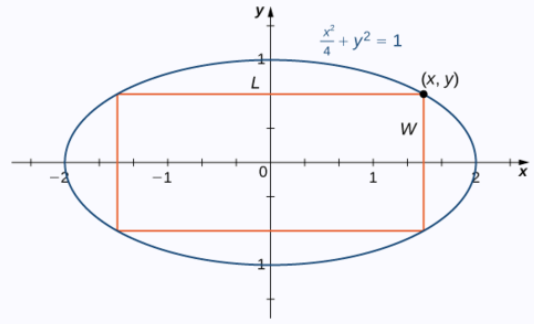
\includegraphics[width=0.9\textwidth]{img/image-20200420234107555.png}

\end{example}
\vspace*{6\baselineskip}

\hypertarget{first-derivative-test-for-absolute-extreme-values}{%
\subsection{First Derivative Test for Absolute Extreme
Values}\label{first-derivative-test-for-absolute-extreme-values}}

\begin{theorem}

Suppose that \(c\) is a critical number of a continuous function \(f\)
defined on an interval.

\begin{enumerate}
\item
  If \(f^{\prime}(x)>0\) for all \(x<c\) and \(f^{\prime}(x)<0\) for all
  \(x>c,\) then \(f(c)\) is the absolute maximum value of \(f\).
\item
  If \(f^{\prime}(x)<0\) for all \(x<c\) and \(f^{\prime}(x)>0\) for all
  \(x>c,\) then \(f(c)\) is the absolute minimum value of \(f\).
\end{enumerate}

\end{theorem}

\begin{example}

A closed box with a square base is to contain 180 cubic feet. The bottom
costs \$4 per square foot, the top costs \$1 per square foot, and the
sides cost \$3 per square foot. Find the dimensions that will minimize
the cost.

\end{example}
\vspace*{6\baselineskip}

\begin{example}

A cylindrical can is to be made to hold 1 L of tomato sauce. Find the
dimensions that will minimize the cost of the metal to manufacture the
can.

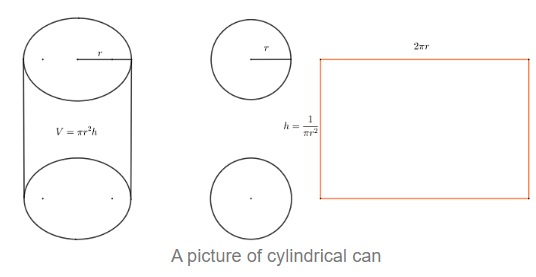
\includegraphics[width=0.9\textwidth]{img/image-20200420234447905.png}

\end{example}
\vspace*{6\baselineskip}

\subsection{Practice}

\begin{exercise}

To carry a suitcase on an airplane, the
\(\text{length} + \text{width} + \text{height}\) of the box must be less
than or equal to 62 in.

\begin{enumerate}
\item
  Assuming the height is fixed, show that the maximum volume is
  \(V=h(31 - (\frac{1}{2})h)^2.\)
\item
  What height allows you to have the largest volume?
\end{enumerate}

\end{exercise}

\begin{exercise}

Two poles are connected by a wire that is also connected to the ground.
The first pole is 20 ft tall and the second pole is 10 ft tall. There is
a distance of 30 ft between the two poles. Where should the wire be
anchored to the ground to minimize the amount of wire needed?

\end{exercise}
\vspace*{6\baselineskip}

\begin{exercise}

For every \(x\) pizzas sold, a pizzeria would make a revenue of
\(R(x)=12x\). It is known that the cost of the pizzeria to make \(x\)
pizzas is \(C(x)=2x+x^2\). How many pizzas sold would maximize the
profit?

\end{exercise}
\vspace*{6\baselineskip}

\begin{exercise}

At where is the parabola \(y=x^2\) closest to point \((0,3)\)?

\end{exercise}
\vspace*{6\baselineskip}

\begin{exercise}

A top-opened cylinder has the volume \(16\pi\). Find the dimensions of
the cylinder that has the least amount of surface area.

\end{exercise}

